\documentclass[12pt,letterpaper]{article}

\usepackage[margin=1in]{geometry} % page margins & stuff
\usepackage{microtype} % improves font readability
\usepackage{yfonts}

\usepackage{hyperref}%adds pdf hyperlinks for document references (e.g., table of contents)
\usepackage{url} % nice url typesetting
\usepackage{textcomp}%used for \textrangle & similar--adds symbols for text environment
\usepackage{graphicx}%for pictures and stuff
\usepackage{subcaption}%needed for side-by-side pictures

\usepackage{multicol}%multicolumn stuff in tables
\usepackage{booktabs}%adds additional table commands (\toprule, etc.)
\usepackage{authblk}%changes the way \author{} works, adds \affiliation{} & similar

\usepackage{hanging}%allows us to use hanging paragraphs in the references section
\usepackage{xcolor}%enables use of colors
\newcommand{\email}[1]{%used to typeset emails in the 'title settings' section
  $\langle$\href{mailto:#1}{\nolinkurl{#1}}$\rangle$
}

\newcommand{\hl}[1] {%used to highlight text
{\color{red}#1}%
}

\title{Proposal for Enhanced Charlottesville Area Transit Mobile Application}
\author{Andrea Shaw \\ \email{rcs8vq@virginia.edu}}%
\affil{Department of Computer Science \\ University of Virginia}

\date{September 2016}

\begin{document}

\maketitle

\begin{abstract}
\hl{Lorem ipsum dolor sit amet, consectetur adipiscing elit. Donec quis semper
    ligula. Nam metus quam, condimentum in leo at, pellentesque pretium ipsum.
    Sed lacus velit, sollicitudin sed turpis non, suscipit feugiat elit. Etiam
    convallis tristique purus, eget tempus leo venenatis id. Curabitur interdum
    semper ante at tristique. Praesent accumsan neque eu justo volutpat
    fermentum. Cras ultricies quam id lorem sodales pulvinar. Curabitur
    ullamcorper ex et sem rhoncus, vel pharetra libero laoreet. Sed dui massa,
    suscipit non sagittis non, imperdiet ac mi. Aliquam fermentum mi et risus
    ullamcorper, non aliquet enim rhoncus. Fusce bibendum pharetra erat eget
    finibus.
}

\bigskip
    \noindent \emph{Keywords}: {\tt Charlottesville Area Transport, public transport, mobile app}
\end{abstract}

\vspace{5mm}

\begin{quote}
A developed country is not a place where the poor have cars. It's where the rich use public transport.

\raggedleft ---attributed to Enrique Pe\~{n}alosa, former Mayor of Bogot\'{a}, Colombia
\end{quote}

\section{Problem Definition}
In 2014, the Charlottesville Area Transit [CAT] organization commissioned a new
mobile app meant to help bus riders better understand their public
transportation options and reduce dependence on the outdated phone-based
timetable system (NBC29 WVIR Charlottesville, 2014). Though basically
functional, the graphical user interface (GUI) of the mobile application leaves
much to be desired. Unlike its web-based counterpart (see Fig.~\ref{fig:cat_online})
the app provides no obvious way of obtaining arrival estimates for all of the
operational area's
bus stops. Furthermore, it may crash or otherwise fail to boot up on many
devices.


\begin{figure}[th!]
    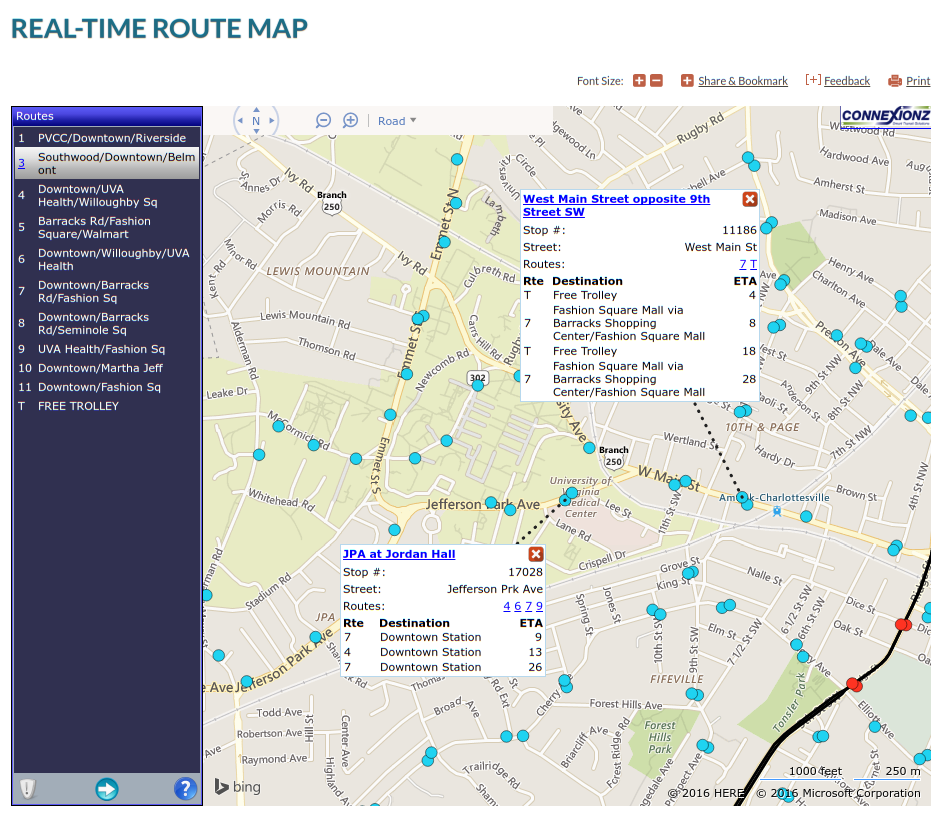
\includegraphics[width=\textwidth]{CAT_online}
    \caption{
        \label{fig:cat_online}
        The CAT ``Real-Time Route Map'', a website designed for desktop
        use that shows a system map, complete with all stops in the service area, along with
        timetable options (City of Charlottesville, n.d.).
    }
\end{figure}

By introducing the arrival estimate system and improving app stability and
design, it is hoped that the application will better serve the
Charlottesville community and increase the individual's access to public
transit. College towns like Charlottesville are relatively unique in that they
often feature a close relationship between schools and the local and municipal
governments that surround them. A result of this mutually-beneficial
arrangement, we find that many college town mass transit options feature unique
challenges.

In the case of Charlottesville, where two primary bus
systems\footnote{The University Transit System (UTS) serves primarily students
and employees of the University of Virginia. The territory covered by
Charlottesville Area Transit overlaps in many cases with that of the UTS---the
CAT Free Trolley, for example, connects the University area to the Downtown
Mall. CAT is also funded, in part, by the University of Virginia (CAT, 2011,
p.~6), and students and ID-carrying employees of the University of Virginia may
ride CAT buses free of charge.} intersect within city limits, the bus-riding
population is significantly more diverse in age and income-level than the country at large.
Whereas riders on CAT bus routes are a steady mix of work-commuters, students,
and shoppers of varying ethnic background (CAT, 2011, p.~48--49), Taylor \&
Morris (2015) contend that bus transit in the United States is generally skewed
towards commuters and minority riders. The limited availability of parking and
other contraindications for travel by car result in a heavy reliance of city
residents from all backgrounds on the bus transit system. It is therefore expedient that
the area continue to invest in the convenience of travel by mass transit for all of
its citizens---their livelihood depends on it.

The improvements suggested in this document to the existing CAT mobile app are hoped to address a broad cross-section
of the community, providing enhanced utility to all users within.

\section{Prototype Brainstorming}
Our proposal suggests implementing minor fixes and \ae{}sthetic tweaks to the existing mobile app. The version current at the time of writing (Charlottesville Area Transit, release 3.8) is displayed in Fig.~\ref{fig:cat_mobile}

\begin{figure}[ph!]
\centering
\begin{subfigure}{.5\textwidth}
  \centering
  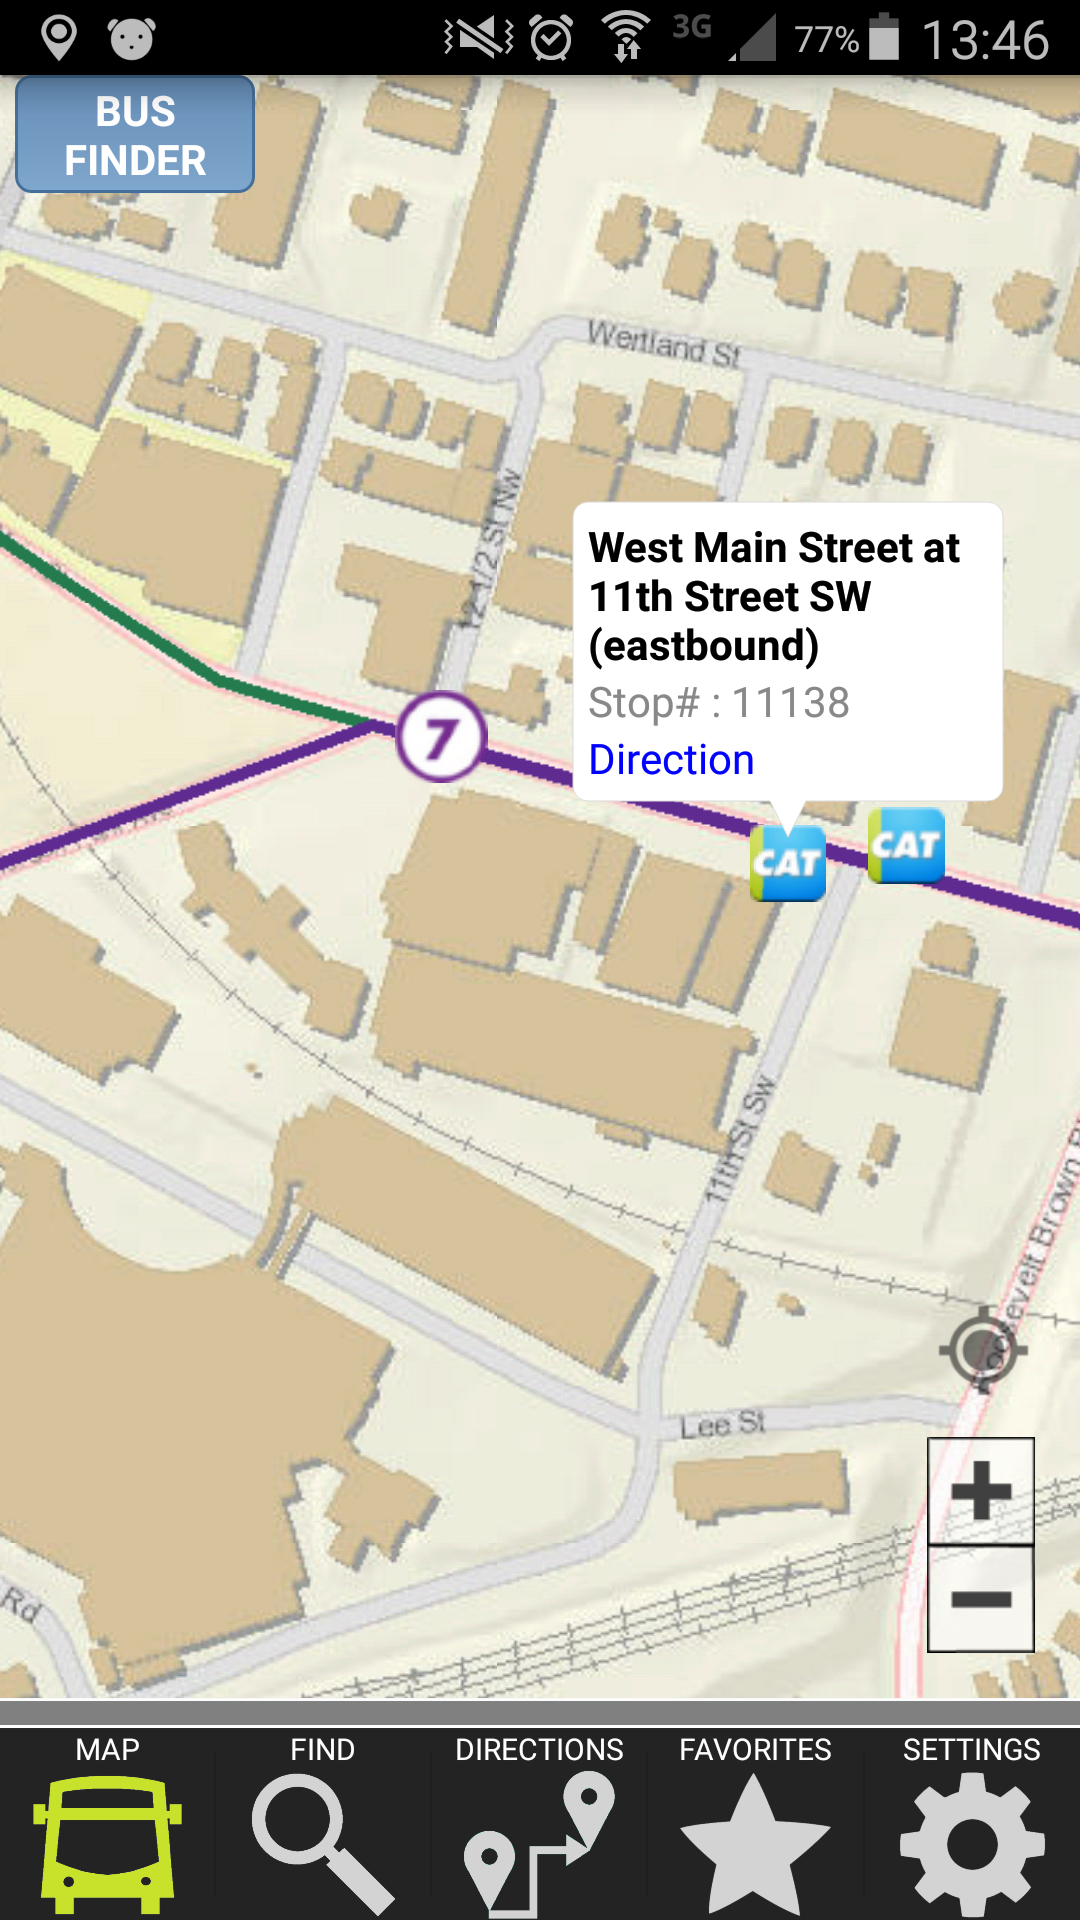
\includegraphics[width=.9\linewidth]{CAT_mobile_1}
  \caption{View of a bus route, stop selected}
  \label{fig:cat_mobile_1}
\end{subfigure}%
\begin{subfigure}{.5\textwidth}
  \centering
  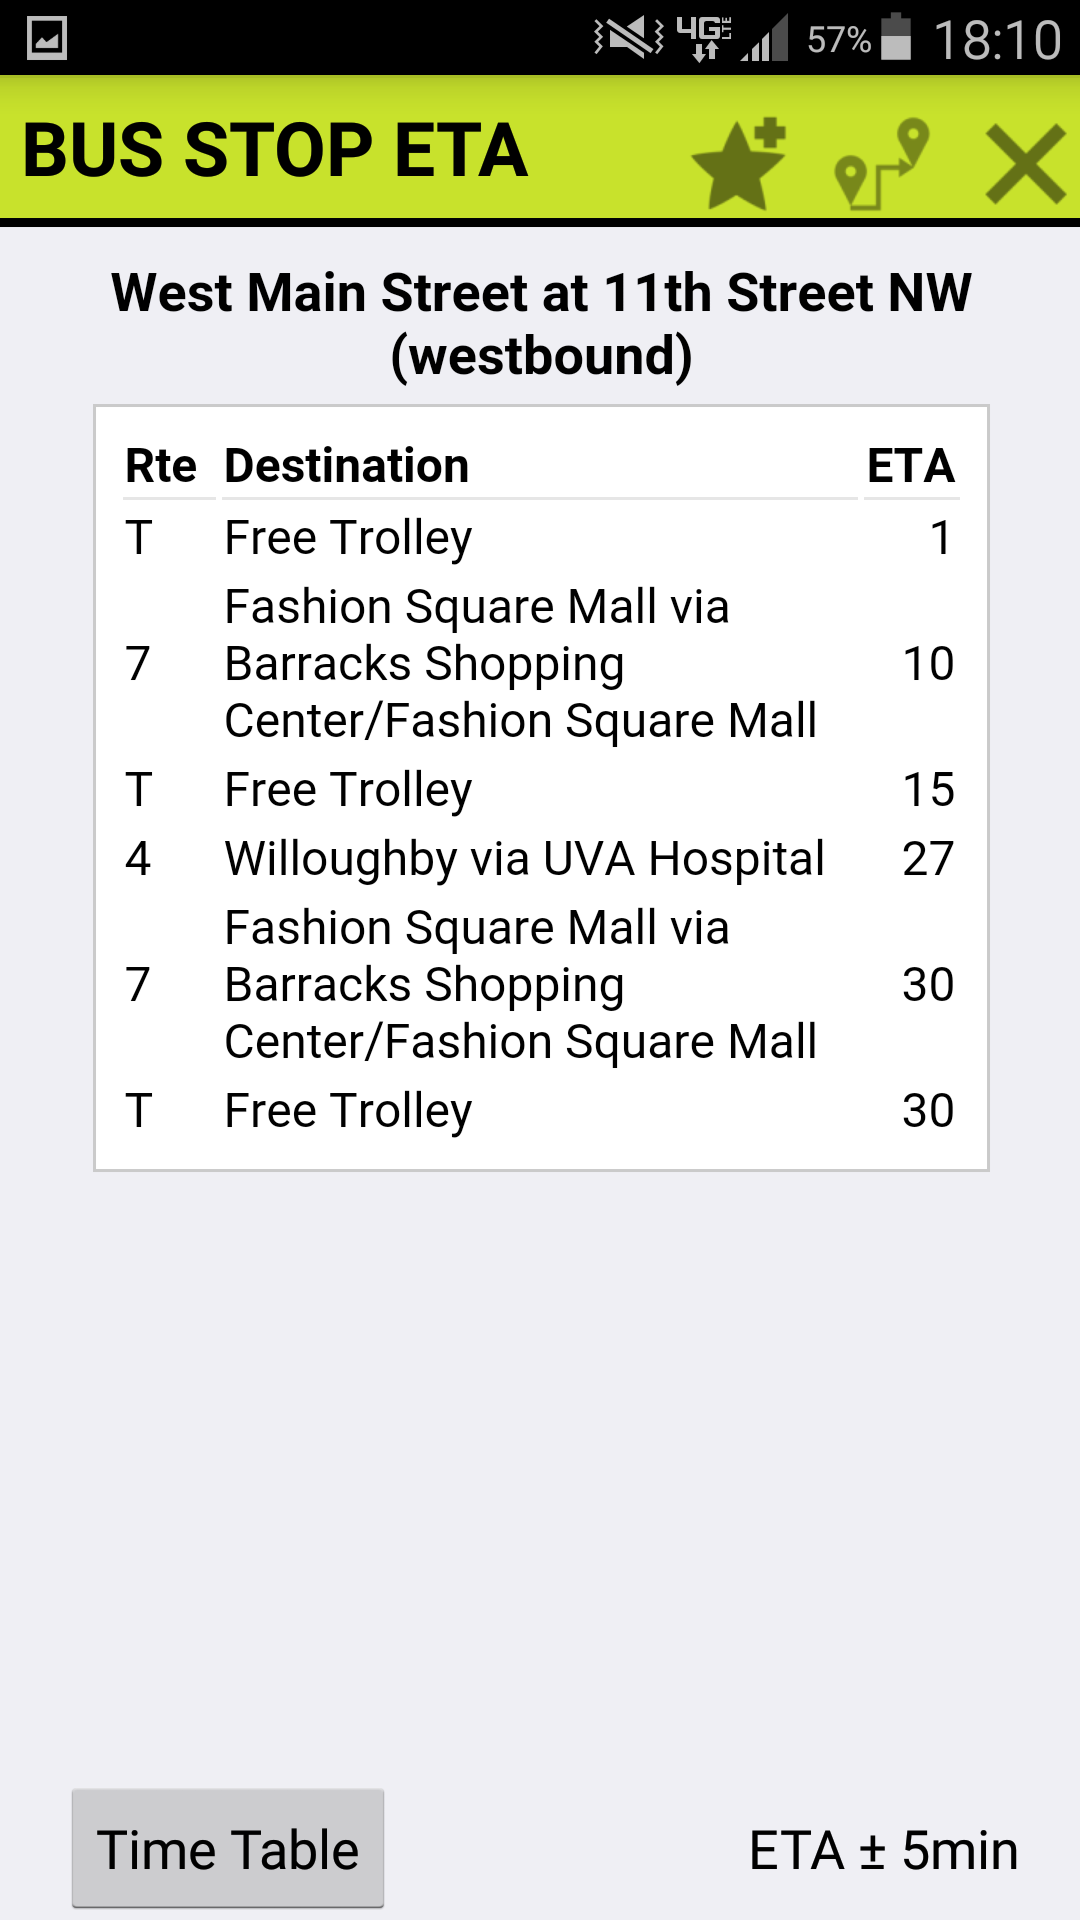
\includegraphics[width=.9\linewidth]{CAT_mobile_2}
  \caption{View of a timetable for the stop}
  \label{fig:cat_mobile_2}
\end{subfigure}
\caption{The Charlottesville Area Transit mobile app, depicted on a Samsung
    Galaxy S4 running Android Lollipop (version 5.0.1). Published by the City of Charlottesville (2016).}
\label{fig:cat_mobile}
\end{figure}

We will categorize this proposal into three areas of development.

\subsection{Modernization of GUI}
Though the current graphical user interface (GUI) for the mobile app is
generally quite functional, some minor cosmetic tweaks are advisable in order
to reduce user cognitive load necessary in learning the application for the
first time. For example, the button display bar at the bottom of the screen
that allows one to switch from one widget to another lacks demarcated borders
between neighboring elements. Additionally, the bar is not readily apparent to
the end user as a functional---they may appear to be part of the route
visualization above.

Our proposed solution to this problem is to redesign these
buttons natively; that is, to utilize the host operating system's pre-existing
(Android, iOS, or other) design features to best familiarize the user with the
app. If funding permits, developers might add on to this integration by
introducing phone notifications when a bus is about to arrive at the
current stop or left-right swiping to switch between one widget and the next.

\subsection{Enhanced Integration of Timetable Feature}
 - TransLoc does it better
 - cite TransLoc app too
 - time table is pretty important!

\subsection{Application Stability}

\section{Expected Results}
\hl{ - poor need public transit the most (Taylor \& Morris, 2015)
What information do you intend to learn from this project? What results do you expect to present? Are you trying to design an interface to maximum profits? To maximize traffic? To minimize frustration? At the end of the semester, what solution will you present and why is it important?

Etiam dapibus ac dui sit amet vestibulum. Nulla faucibus odio vel augue ultrices, non eleifend sapien suscipit. Pellentesque rutrum, leo ut lobortis ornare, odio augue mattis eros, sit amet tristique quam elit nec nibh. Proin lacinia sollicitudin ullamcorper. Fusce fermentum vitae orci ut feugiat. Class aptent taciti sociosqu ad litora torquent per conubia nostra, per inceptos himenaeos. Ut vitae massa libero. Integer dictum consequat neque posuere pretium. Nulla sed ligula sodales, ultrices quam a, elementum nunc. In in orci quis nisl varius euismod. Quisque lobortis mauris et porta dapibus. Etiam sed erat vehicula, consectetur arcu ac, venenatis orci. Morbi dapibus est eget mauris auctor pulvinar. Curabitur at leo vel arcu sollicitudin scelerisque a in eros. Duis sit amet blandit mi, ac luctus felis. Vestibulum sodales efficitur ex, ac dictum lorem rhoncus ac.
}

\section{Acknowledgements}
The author wishes to recognize Luther Tychonievich, Ph.D, lecturer at the
University of Virginia, for his seminars introducing basic
cognitive load theory, which heavily influenced the changes suggested in this
proposal.

\section{Honor Code}
On my word of honor, I have neither given nor received any unauthorized aid on this assignment.
\begin{center}
    Andrea Shaw\qquad {\hrulefill} \qquad 2016--08--25
\end{center}

\section{References}
\hangparas{1cm}{1}
Charlottesville Area Transit (2011, May). Transit Development Plan: Fiscal Years 2012--2017. Retrieved from \href{http://drpt.virginia.gov/media/1482/charlottesville-area-transit.pdf}{\tt http://drpt.virginia.gov/media/1482/charlottesville-area- \\
transit.pdf}.

City of Charlottesville (n.d.). Real-time Route Map. Retrieved from \href{http://www.charlottesville.org/departments-and-services/city-services/charlottesville-area-transit-cat/real-time-route-map}{\tt http:// \\
charlottesville.org/departments-and-services/ciity-services/ \\
charlottesville-area-transit-cat/real-time-route-map}.

City of Charlottesville (2016, 23 May). Charlottesville Area Transit (version 3.8) [Mobile application software]. Retrieved from \url{https://play.google.com/store/apps/details?id=com.cville.cattail}.

NBC29 WVIR Charlottesville (2014, 28 February). CAT riders can monitor bus status with new app. Retrieved online from \url{http://www.nbc29.com/story/24856561/cat-riders-can-monitor-bus-status-with-new-app}.

Taylor, B.D. \& Morris, E.A. Transportation (2015) Public transportation objectives and rider demographics:
are transit’s priorities poor public policy? \emph{Transportation}, 42, 347--367. doi:10.1007/s11116-014-9547-0
\end{document}

